\documentclass[11pt,]{article}
\usepackage[left=1in,top=1in,right=1in,bottom=1in]{geometry}
\newcommand*{\authorfont}{\fontfamily{phv}\selectfont}
\usepackage[]{mathpazo}


  \usepackage[T1]{fontenc}
  \usepackage[utf8]{inputenc}




\usepackage{abstract}
\renewcommand{\abstractname}{}    % clear the title
\renewcommand{\absnamepos}{empty} % originally center

\renewenvironment{abstract}
 {{%
    \setlength{\leftmargin}{0mm}
    \setlength{\rightmargin}{\leftmargin}%
  }%
  \relax}
 {\endlist}

\makeatletter
\def\@maketitle{%
  \newpage
%  \null
%  \vskip 2em%
%  \begin{center}%
  \let \footnote \thanks
    {\fontsize{18}{20}\selectfont\raggedright  \setlength{\parindent}{0pt} \@title \par}%
}
%\fi
\makeatother




\setcounter{secnumdepth}{0}

\usepackage{color}
\usepackage{fancyvrb}
\newcommand{\VerbBar}{|}
\newcommand{\VERB}{\Verb[commandchars=\\\{\}]}
\DefineVerbatimEnvironment{Highlighting}{Verbatim}{commandchars=\\\{\}}
% Add ',fontsize=\small' for more characters per line
\usepackage{framed}
\definecolor{shadecolor}{RGB}{248,248,248}
\newenvironment{Shaded}{\begin{snugshade}}{\end{snugshade}}
\newcommand{\AlertTok}[1]{\textcolor[rgb]{0.94,0.16,0.16}{#1}}
\newcommand{\AnnotationTok}[1]{\textcolor[rgb]{0.56,0.35,0.01}{\textbf{\textit{#1}}}}
\newcommand{\AttributeTok}[1]{\textcolor[rgb]{0.77,0.63,0.00}{#1}}
\newcommand{\BaseNTok}[1]{\textcolor[rgb]{0.00,0.00,0.81}{#1}}
\newcommand{\BuiltInTok}[1]{#1}
\newcommand{\CharTok}[1]{\textcolor[rgb]{0.31,0.60,0.02}{#1}}
\newcommand{\CommentTok}[1]{\textcolor[rgb]{0.56,0.35,0.01}{\textit{#1}}}
\newcommand{\CommentVarTok}[1]{\textcolor[rgb]{0.56,0.35,0.01}{\textbf{\textit{#1}}}}
\newcommand{\ConstantTok}[1]{\textcolor[rgb]{0.00,0.00,0.00}{#1}}
\newcommand{\ControlFlowTok}[1]{\textcolor[rgb]{0.13,0.29,0.53}{\textbf{#1}}}
\newcommand{\DataTypeTok}[1]{\textcolor[rgb]{0.13,0.29,0.53}{#1}}
\newcommand{\DecValTok}[1]{\textcolor[rgb]{0.00,0.00,0.81}{#1}}
\newcommand{\DocumentationTok}[1]{\textcolor[rgb]{0.56,0.35,0.01}{\textbf{\textit{#1}}}}
\newcommand{\ErrorTok}[1]{\textcolor[rgb]{0.64,0.00,0.00}{\textbf{#1}}}
\newcommand{\ExtensionTok}[1]{#1}
\newcommand{\FloatTok}[1]{\textcolor[rgb]{0.00,0.00,0.81}{#1}}
\newcommand{\FunctionTok}[1]{\textcolor[rgb]{0.00,0.00,0.00}{#1}}
\newcommand{\ImportTok}[1]{#1}
\newcommand{\InformationTok}[1]{\textcolor[rgb]{0.56,0.35,0.01}{\textbf{\textit{#1}}}}
\newcommand{\KeywordTok}[1]{\textcolor[rgb]{0.13,0.29,0.53}{\textbf{#1}}}
\newcommand{\NormalTok}[1]{#1}
\newcommand{\OperatorTok}[1]{\textcolor[rgb]{0.81,0.36,0.00}{\textbf{#1}}}
\newcommand{\OtherTok}[1]{\textcolor[rgb]{0.56,0.35,0.01}{#1}}
\newcommand{\PreprocessorTok}[1]{\textcolor[rgb]{0.56,0.35,0.01}{\textit{#1}}}
\newcommand{\RegionMarkerTok}[1]{#1}
\newcommand{\SpecialCharTok}[1]{\textcolor[rgb]{0.00,0.00,0.00}{#1}}
\newcommand{\SpecialStringTok}[1]{\textcolor[rgb]{0.31,0.60,0.02}{#1}}
\newcommand{\StringTok}[1]{\textcolor[rgb]{0.31,0.60,0.02}{#1}}
\newcommand{\VariableTok}[1]{\textcolor[rgb]{0.00,0.00,0.00}{#1}}
\newcommand{\VerbatimStringTok}[1]{\textcolor[rgb]{0.31,0.60,0.02}{#1}}
\newcommand{\WarningTok}[1]{\textcolor[rgb]{0.56,0.35,0.01}{\textbf{\textit{#1}}}}
\usepackage{longtable,booktabs}

\usepackage{graphicx,grffile}
\makeatletter
\def\maxwidth{\ifdim\Gin@nat@width>\linewidth\linewidth\else\Gin@nat@width\fi}
\def\maxheight{\ifdim\Gin@nat@height>\textheight\textheight\else\Gin@nat@height\fi}
\makeatother
% Scale images if necessary, so that they will not overflow the page
% margins by default, and it is still possible to overwrite the defaults
% using explicit options in \includegraphics[width, height, ...]{}
\setkeys{Gin}{width=\maxwidth,height=\maxheight,keepaspectratio}


\title{Predicting House Prices in Toronto: A Machine Learning Approach  }



\author{\Large Albina Cako, BSc\vspace{0.05in} \newline\normalsize\emph{York University, Certificate in Machine Learning}   \and \Large Colin Green, BSc\vspace{0.05in} \newline\normalsize\emph{York University, Certificate in Machine Learning}   \and \Large Lucy Zhang, BSc\vspace{0.05in} \newline\normalsize\emph{York University, Certificate in Machine Learning}   \and \Large Sean X. Zhang, MSc\vspace{0.05in} \newline\normalsize\emph{York University, Certificate in Machine Learning}  }


\date{}

\usepackage{titlesec}

\titleformat*{\section}{\normalsize\bfseries}
\titleformat*{\subsection}{\normalsize\itshape}
\titleformat*{\subsubsection}{\normalsize\itshape}
\titleformat*{\paragraph}{\normalsize\itshape}
\titleformat*{\subparagraph}{\normalsize\itshape}





\newtheorem{hypothesis}{Hypothesis}
\usepackage{setspace}


% set default figure placement to htbp
\makeatletter
\def\fps@figure{htbp}
\makeatother

\usepackage{booktabs}
\usepackage{longtable}
\usepackage{array}
\usepackage{multirow}
\usepackage{wrapfig}
\usepackage{float}
\usepackage{colortbl}
\usepackage{pdflscape}
\usepackage{tabu}
\usepackage{threeparttable}
\usepackage{threeparttablex}
\usepackage[normalem]{ulem}
\usepackage{makecell}
\usepackage{xcolor}

% move the hyperref stuff down here, after header-includes, to allow for - \usepackage{hyperref}

\makeatletter
\@ifpackageloaded{hyperref}{}{%
\ifxetex
  \PassOptionsToPackage{hyphens}{url}\usepackage[setpagesize=false, % page size defined by xetex
              unicode=false, % unicode breaks when used with xetex
              xetex]{hyperref}
\else
  \PassOptionsToPackage{hyphens}{url}\usepackage[draft,unicode=true]{hyperref}
\fi
}

\@ifpackageloaded{color}{
    \PassOptionsToPackage{usenames,dvipsnames}{color}
}{%
    \usepackage[usenames,dvipsnames]{color}
}
\makeatother
\hypersetup{breaklinks=true,
            bookmarks=true,
            pdfauthor={Albina Cako, BSc (York University, Certificate in Machine Learning) and Colin Green, BSc (York University, Certificate in Machine Learning) and Lucy Zhang, BSc (York University, Certificate in Machine Learning) and Sean X. Zhang, MSc (York University, Certificate in Machine Learning)},
             pdfkeywords = {house prices, machine learning, caret, shiny},  
            pdftitle={Predicting House Prices in Toronto: A Machine Learning Approach},
            colorlinks=true,
            citecolor=blue,
            urlcolor=blue,
            linkcolor=magenta,
            pdfborder={0 0 0}}
\urlstyle{same}  % don't use monospace font for urls

% Add an option for endnotes. -----


% add tightlist ----------
\providecommand{\tightlist}{%
\setlength{\itemsep}{0pt}\setlength{\parskip}{0pt}}

% add some other packages ----------

% \usepackage{multicol}
% This should regulate where figures float
% See: https://tex.stackexchange.com/questions/2275/keeping-tables-figures-close-to-where-they-are-mentioned
\usepackage[section]{placeins}


\begin{document}
	
% \pagenumbering{arabic}% resets `page` counter to 1 
%
% \maketitle

{% \usefont{T1}{pnc}{m}{n}
\setlength{\parindent}{0pt}
\thispagestyle{plain}
{\fontsize{18}{20}\selectfont\raggedright 
\maketitle  % title \par  

}

{
   \vskip 13.5pt\relax \normalsize\fontsize{11}{12} 
\textbf{\authorfont Albina Cako, BSc} \hskip 15pt \emph{\small York University, Certificate in Machine Learning}   \par \textbf{\authorfont Colin Green, BSc} \hskip 15pt \emph{\small York University, Certificate in Machine Learning}   \par \textbf{\authorfont Lucy Zhang, BSc} \hskip 15pt \emph{\small York University, Certificate in Machine Learning}   \par \textbf{\authorfont Sean X. Zhang, MSc} \hskip 15pt \emph{\small York University, Certificate in Machine Learning}   

}

}








\begin{abstract}

    \hbox{\vrule height .2pt width 39.14pc}

    \vskip 8.5pt % \small 

\noindent The project focus on building a machine learning model for predicting
house price in Toronto. Although House Price Index (HPI) is commonly
used for estimating the changes in housing price but it is not perfect
for individual housing price prediction due to high correlation of
housing price and other factors such as house location, income
distribution, area, and etc. This project evaluates four different model
and chooses the best one for deployment with ShinyApp. The app created
for both buyer and seller to have an estimated house price due the
location and different attributes of the house, and help users to make
decisions.


\vskip 8.5pt \noindent \emph{Keywords}: house prices, machine learning, caret, shiny \par

    \hbox{\vrule height .2pt width 39.14pc}



\end{abstract}


\vskip -8.5pt


 % removetitleabstract

\noindent  

\hypertarget{introduction}{%
\section{Introduction}\label{introduction}}

The House Pricing Prediction app is created for estimate the house price
for both buyer and seller based on different factors such as total Sqft,
house locations, etc. The deployment was constructed using ShinyApp. An
user friendly app for both buyer and seller, with simple click of
factors users will get an estimated housing price. The app can be used
for individual buyers who want to know the final price of the houses
they are interested or for individual sellers to know what is the best
listing price. The app uses regression model for prediction, which was
trained by the data set of Toronto housing price. The housing price is
strongly correlated with other factors, for increasing the model
accuracy decreasing errors, it is important to try different factors and
combinations. This project will comprehensively validate four different
models: decision tree, random forest, K nearest neighbors, and gradient
boosting machine. This report will go through data analysis, modeling
implementation and provide an optimistic result for housing price
prediction.

\hypertarget{objective}{%
\subsection{Objective}\label{objective}}

The objective of this project was to evaluate the application of machine
learning algorithms to predict house prices in the Greater Toronto Area,
and apply

\hypertarget{background}{%
\subsection{Background}\label{background}}

Purchasing a house is a big life decision for every individual and needs
a considerable amount of research. Everyone has different purpose of
buying houses, someone would prefer by the house at the best rate for
living now, someone would buy houses for future investment. Selling the
houses is also very important and needs to do research and decide what
is the best leasing price. Commonly, people will ask advise from various
websites, real estate agents or realtors before purchasing or leasing;
However, due to the trend towards big data, house pricing prediction can
be done by using machine learning strategies base on large amount of
data from previous years more correctly. House Price Index (HPI) can
measure the price changes of residential housing as a percentage change,
In Canada the new Housing Price Index is calculated monthly by
Statistics Canada. HPI is useful but because it is a rough indicator
calculated from all transactions, it is inefficient for predicting a
specific house with its attributes. The purpose of this project is to
create an app for both buyers and sellers can easily check the predicted
list price or final price based on the attributes of the house such as
locations, square foot, number of bedrooms, etc.

\hypertarget{methodology}{%
\section{Methodology}\label{methodology}}

\hypertarget{data-preprocessing}{%
\subsection{Data Preprocessing}\label{data-preprocessing}}

The housing dataset, originally shared on Github{[}1{]}, was extracted
from Zoocasa.com in the summer of 2019. The dataset contained all
completed property sales in the city of Toronto within an approximately
1-year span. We performed several data exploration and cleaning steps to
prepare this data for modeling.

\hypertarget{missingness}{%
\subsection{Missingness}\label{missingness}}

We assessed the dataset for missing values. Many parametric machine
learning models do not accept missing data, and the accuracy of even
non-parametric models are often negatively impacted by missingness.
Thus, missing values ought to be either imputed or removed before data
modeling. We then determined whether missing data was Missing Completely
at Random (MCAR), Missing at Random (MAR), or Missing Not at Random
(MNAR). Should the data be MCAR, then it is acceptable to simply remove
each observation that is missing, as doing so would not introduce bias
to the remaining observations. However, if there was a correlation
between missingness and other data features, then imputation must be
performed. Missingness correlation was assessed using the
missing\_compare() function from the finalfit library, which applies the
Kruskal Wallis correlation test for numerical variables and chi-squared
correlation test for categorical variables to determine correlation.
Using the MICE package in R, we then applied the following imputation
methods: 1) simple, which imputes a value from a simple random sample
from the rest of the data; 2) mean, which imputes the average of all
observations; 3) random forest, which applies a random forest algorithm;
and 4) CART, which imputes by classification and regression trees. The
distribution of the imputed data were evaluated with a density plot and
an imputed dataset was chosen based on best fit.

\hypertarget{data-curation}{%
\subsection{Data Curation}\label{data-curation}}

\hypertarget{modeling}{%
\subsection{Modeling}\label{modeling}}

As the data contained a mix of categorical and numerical variables and
did not satisfy many requirements of parametric models, such as variable
independence, and normally distributed data. Thus, several parametric
models were used. We trained four different non-parametric models using
k-fold cross validation. The models were then tuned using various grid
searches to improve the accuracy. The final model was chosen based on
three metrics: Root Mean-Squared Error (RMSE), Pearson correlation
(R\^{}2), and Mean Average Error (MAE).

\hypertarget{decision-tree-model}{%
\subsubsection{\texorpdfstring{\textbf{Decision Tree Model}\\
}{Decision Tree Model }}\label{decision-tree-model}}

\textless\textless\textless\textless\textless\textless\textless{} HEAD
\#\# Data Preprocessing The housing dataset, originally shared on
Github{[}1{]}, was extracted from Zoocasa.com in the summer of 2019. The
dataset contained all completed property sales in the city of Toronto
within a 1-year span. We performed several data exploration and cleaning
steps to prepare this data for modeling.

\hypertarget{missingness-1}{%
\subsection{Missingness}\label{missingness-1}}

We assessed the dataset for missing values. Many parametric machine
learning models do not accept missing data, and the accuracy of even
non-parametric models are often negatively impacted by missingness.
Thus, missing values ought to be either imputed or removed before data
modeling. We then determined whether missing data was Missing Completely
at Random (MCAR), Missing at Random (MAR), or Missing Not at Random
(MNAR). Should the data be MCAR, then it is acceptable to simply remove
each observation that is missing, as doing so would not introduce bias
to the remaining observations. However, if there was a correlation
between missingness and other data features, then imputation must be
performed. Missingness correlation was assessed using the
missing\_compare() function from the finalfit library, which applies the
Kruskal Wallis correlation test for numerical variables and chi-squared
correlation test for categorical variables to determine correlation.
Using the MICE package in R, we then applied the following imputation
methods: 1) simple, which imputes a value from a simple random sample
from the rest of the data; 2) mean, which imputes the average of all
observations; 3) random forest, which applies a random forest algorithm;
and 4) CART, which imputes by classification and regression trees. The
distribution of the imputed data were evaluated with a density plot and
an imputed dataset was chosen based on best fit.

\hypertarget{assessing-parametric-fit}{%
\subsection{Assessing Parametric Fit}\label{assessing-parametric-fit}}

Outliers were visualized with the boxplot() function. Data were
considered outliers if they were less than Q1 - 1.5 X Inter-Quartile
Range and greater Q3 + 1.5 X Inter-Quartile Range. Normality of the
distribution of variables were visualized with density plots. A
correlogram with Pearson's R determined collinearity. Linear
relationship between outcome variable and predictors was tested via
scatterplots.

\hypertarget{data-curation-1}{%
\subsection{Data Curation}\label{data-curation-1}}

The following variables were removed as they did not have any data
utility or were not easily parseable (i.e.~free text): title,
description, mls, type, full\_link, full\_address. A numeric `bedrooms'
column was created by combining bedrooms\_ag and bedrooms\_bg. We also
removed district\_code and city\_district. Both were categorical
variables with number of factors = 140; keeping these would
significantly increase model training time. We also did not consider
longitude and latitude, as including these variables in training sets
would have required geocoding and district clustering; complexities
which were outside our scope for this application.
Mean\_district\_income was left as an approximation of the effect of
districts on property price. After consultation with a real-estate
expert, we decreased the number of property types by generalizing types
to: Townhouse, Condo, Detached, Semi-Detached, and Plex. Thus, the
predictors chosen were:

\begin{longtable}[]{@{}lll@{}}
\caption{Predictor variables}\tabularnewline
\toprule
Label & & Description\tabularnewline
\midrule
\endfirsthead
\toprule
Label & & Description\tabularnewline
\midrule
\endhead
sqft & & numeric\tabularnewline
beds & & numeric\tabularnewline
bathrooms & & numeric\tabularnewline
parking & & numeric\tabularnewline
mean\_district\_income & & numeric\tabularnewline
type & & categorical\tabularnewline
\bottomrule
\end{longtable}

The target variable chosen was final\_price. The dataset also contained
a list\_price variable. Rather than training two models to predict on
both list and final price, the predicted list price was instead
approximated by a linear equation between list and final price from the
original dataset.

\hypertarget{modeling-1}{%
\subsection{Modeling}\label{modeling-1}}

The data contained a mix of categorical and numerical variables. These
variables did not satisfy the many requirements of parametric models,
such as variable independence, normally distributed data, and linear
relationship with outcome. Thus, several non-parametric models were used
instead. We trained four different models using k-fold cross validation.
The models were then tuned using various grid searches to improve the
accuracy. The final model was then chosen based on three accuracy
metrics: Root Mean-Squared Error (RMSE), Pearson correlation (R\^{}2),
and Mean Average Error (MAE).

\begin{verbatim}
## Warning in kable_styling(mtable, font_size = 10): Please specify format in
## kable. kableExtra can customize either HTML or LaTeX outputs. See https://
## haozhu233.github.io/kableExtra/ for details.
\end{verbatim}

\begin{longtable}[]{@{}lll@{}}
\caption{Non-parametric Models Used}\tabularnewline
\toprule
\begin{minipage}[b]{0.05\columnwidth}\raggedright
Model\strut
\end{minipage} & \begin{minipage}[b]{0.73\columnwidth}\raggedright
Description\strut
\end{minipage} & \begin{minipage}[b]{0.13\columnwidth}\raggedright
Tuning parameters\strut
\end{minipage}\tabularnewline
\midrule
\endfirsthead
\toprule
\begin{minipage}[b]{0.05\columnwidth}\raggedright
Model\strut
\end{minipage} & \begin{minipage}[b]{0.73\columnwidth}\raggedright
Description\strut
\end{minipage} & \begin{minipage}[b]{0.13\columnwidth}\raggedright
Tuning parameters\strut
\end{minipage}\tabularnewline
\midrule
\endhead
\begin{minipage}[t]{0.05\columnwidth}\raggedright
Decision\strut
\end{minipage} & \begin{minipage}[t]{0.73\columnwidth}\raggedright
\strut
\end{minipage} & \begin{minipage}[t]{0.13\columnwidth}\raggedright
\strut
\end{minipage}\tabularnewline
\begin{minipage}[t]{0.05\columnwidth}\raggedright
Tree\strut
\end{minipage} & \begin{minipage}[t]{0.73\columnwidth}\raggedright
Decision trees repeatedly partition data at specific nodes until the
data at the bottom of each branch (known as a leaf) is as homogenous as
possible. The model increases in complexity with each additional
partition and subsequently becomes more accurate.\strut
\end{minipage} & \begin{minipage}[t]{0.13\columnwidth}\raggedright
cp (complexity)\strut
\end{minipage}\tabularnewline
\begin{minipage}[t]{0.05\columnwidth}\raggedright
Random\strut
\end{minipage} & \begin{minipage}[t]{0.73\columnwidth}\raggedright
\strut
\end{minipage} & \begin{minipage}[t]{0.13\columnwidth}\raggedright
\strut
\end{minipage}\tabularnewline
\begin{minipage}[t]{0.05\columnwidth}\raggedright
Forest\strut
\end{minipage} & \begin{minipage}[t]{0.73\columnwidth}\raggedright
Random Forest Model Random Forests are an ensemble learning method for
classification and regression. This method will construct a multitude of
decision trees and output the mean/average prediction problem for
regression or the classes for classification problem. The algorithm can
control the number of variable available for splitting at each tree or
the number of trees to get a higher accuracy.\strut
\end{minipage} & \begin{minipage}[t]{0.13\columnwidth}\raggedright
ntree, mtry\strut
\end{minipage}\tabularnewline
\begin{minipage}[t]{0.05\columnwidth}\raggedright
Gradient Boosting\strut
\end{minipage} & \begin{minipage}[t]{0.73\columnwidth}\raggedright
\strut
\end{minipage} & \begin{minipage}[t]{0.13\columnwidth}\raggedright
\strut
\end{minipage}\tabularnewline
\begin{minipage}[t]{0.05\columnwidth}\raggedright
Machines\strut
\end{minipage} & \begin{minipage}[t]{0.73\columnwidth}\raggedright
Gradient Boosting Machines (gbm) begin with creating a preliminary `weak
learner' decision tree, then sequentially grows more trees that aim to
reduce the error of the last one. The algorithm optimizes the loss
function by minimizing the residuals at each iteration (difference
between predicted and actual value).\strut
\end{minipage} & \begin{minipage}[t]{0.13\columnwidth}\raggedright
n.trees, shrinkage, interaction.depth, n.minobssinnode\strut
\end{minipage}\tabularnewline
\begin{minipage}[t]{0.05\columnwidth}\raggedright
XGBoost\strut
\end{minipage} & \begin{minipage}[t]{0.73\columnwidth}\raggedright
XGBoost uses ensemble learning, which is a systematic solution that
combines the predictive power of multiple learners. It outputs a single
model that gives the combined output from many models. This allows the
opportunity to not rely on the results of a single machine learning
model. In this particular model, the trees are built sequentially, such
that the next tree focuses on reducing the errors of the previous
tree.\strut
\end{minipage} & \begin{minipage}[t]{0.13\columnwidth}\raggedright
nrounds, max\_depth, eta, gamma, colsample\_bytree, min\_child\_weight,
subsample\strut
\end{minipage}\tabularnewline
\bottomrule
\end{longtable}

\hypertarget{deployment}{%
\subsection{Deployment}\label{deployment}}

\hypertarget{the-application-was-created-using-r-shiny-and-hosted-on-the-shinyapps.io-cloud.-edit-this-could-probably-all-go-to-results-section-the-user-interface-ui-contains-a-map-of-toronto-for-geographic-navigation-and-also-allows-the-user-to-select-various-inputs-to-predict-property-price.-while-the-user-would-choose-a-district-of-interest-from-the-front-end-the-back-end-links-the-district-chosen-with-income-and-uses-mean_district_income-as-the-model-input-instead.-we-chose-insert_model-here-since-it-was-the-most-accurate-model-as-the-back-end-for-our-application.}{%
\section{The application was created using R shiny and hosted on the
Shinyapps.io cloud. EDIT : this could probably all go to results section
--\textgreater{} The user interface (UI) contains a map of Toronto for
geographic navigation and also allows the user to select various inputs
to predict property price. While the user would choose a district of
interest from the front end, the back end links the district chosen with
income and uses mean\_district\_income as the model input instead. We
chose INSERT\_MODEL HERE, since it was the most accurate model as the
back-end for our
application.}\label{the-application-was-created-using-r-shiny-and-hosted-on-the-shinyapps.io-cloud.-edit-this-could-probably-all-go-to-results-section-the-user-interface-ui-contains-a-map-of-toronto-for-geographic-navigation-and-also-allows-the-user-to-select-various-inputs-to-predict-property-price.-while-the-user-would-choose-a-district-of-interest-from-the-front-end-the-back-end-links-the-district-chosen-with-income-and-uses-mean_district_income-as-the-model-input-instead.-we-chose-insert_model-here-since-it-was-the-most-accurate-model-as-the-back-end-for-our-application.}}

\begin{quote}
\begin{quote}
\begin{quote}
\begin{quote}
\begin{quote}
\begin{quote}
\begin{quote}
44c2ed0c3345e5e8d262ee90e1917aa199875ab4
\end{quote}
\end{quote}
\end{quote}
\end{quote}
\end{quote}
\end{quote}
\end{quote}

\hypertarget{results}{%
\section{Results}\label{results}}

The original housing dataset contained 21 variables and 15234
observations. Table 1 defines each variable of the dataset.

\begin{longtable}[]{@{}lll@{}}
\caption{Data Dictionary}\tabularnewline
\toprule
Variable & & Type\tabularnewline
\midrule
\endfirsthead
\toprule
Variable & & Type\tabularnewline
\midrule
\endhead
title & & Title of the listing\tabularnewline
final\_price & & Final price of the property\tabularnewline
list\_price & & Listing price of the property\tabularnewline
bedrooms & & Number of bedrooms\tabularnewline
bathrooms & & Number of bathrooms\tabularnewline
sqft & & Area of property in square feet\tabularnewline
parking & & Number of parking spaces\tabularnewline
description & & Verbatim text description of the property\tabularnewline
mls & & MLS Listing ID\tabularnewline
type & & Property type\tabularnewline
full\_link & & URL to listing\tabularnewline
full\_address & & Full address of the property\tabularnewline
lat & & Latitude\tabularnewline
long & & Longitude\tabularnewline
city\_district & & Toronto district to which property belonged
to\tabularnewline
mean\_district\_income & & Average household income of
district\tabularnewline
district\_code & & Numerical code of the district\tabularnewline
final\_price\_transformed & & Box-Cox transformation of final
price\tabularnewline
final\_price\_log & & Log transformation of final price\tabularnewline
bedrooms\_ag & & Number of bedrooms above ground\tabularnewline
bedrooms\_bg & & Number of bedrooms below ground\tabularnewline
\bottomrule
\end{longtable}

\hypertarget{data-exploration}{%
\subsection{Data Exploration}\label{data-exploration}}

\begin{Shaded}
\begin{Highlighting}[]
\NormalTok{data <-}\StringTok{ }\KeywordTok{read.csv}\NormalTok{(}\StringTok{'houses_edited.csv'}\NormalTok{)}
\NormalTok{numeric_cols <-}\StringTok{ }\KeywordTok{list}\NormalTok{(}\StringTok{'final_price'}\NormalTok{, }\StringTok{'list_price'}\NormalTok{, }\StringTok{'bathrooms'}\NormalTok{, }\StringTok{'sqft'}\NormalTok{, }\StringTok{'parking'}\NormalTok{, }\StringTok{'lat'}\NormalTok{, }\StringTok{'long'}\NormalTok{, }\StringTok{'mean_district_income'}\NormalTok{, }\StringTok{'bedrooms_ag'}\NormalTok{, }\StringTok{'bedrooms_bg'}\NormalTok{)}
\NormalTok{predictor_cols <-}\StringTok{ }\KeywordTok{list}\NormalTok{(}\StringTok{'bathrooms'}\NormalTok{, }\StringTok{'sqft'}\NormalTok{, }\StringTok{'parking'}\NormalTok{, }\StringTok{'lat'}\NormalTok{, }\StringTok{'long'}\NormalTok{, }\StringTok{'mean_district_income'}\NormalTok{, }\StringTok{'bedrooms_ag'}\NormalTok{, }\StringTok{'bedrooms_bg'}\NormalTok{)}
\end{Highlighting}
\end{Shaded}

\hypertarget{section}{%
\subsubsection{}\label{section}}

\begin{Shaded}
\begin{Highlighting}[]
\CommentTok{#histograms - note skew in prices}
\KeywordTok{par}\NormalTok{(}\DataTypeTok{mfrow=}\KeywordTok{c}\NormalTok{(}\DecValTok{2}\NormalTok{, }\DecValTok{5}\NormalTok{))}
\ControlFlowTok{for}\NormalTok{ (i }\ControlFlowTok{in}\NormalTok{ numeric_cols) \{}
  \KeywordTok{hist}\NormalTok{(data[[i]], }\DataTypeTok{main =} \KeywordTok{paste}\NormalTok{(i), }\DataTypeTok{xlab =} \StringTok{''}\NormalTok{, }\DataTypeTok{col =} \DecValTok{4}\NormalTok{)}
\NormalTok{\}}
\end{Highlighting}
\end{Shaded}

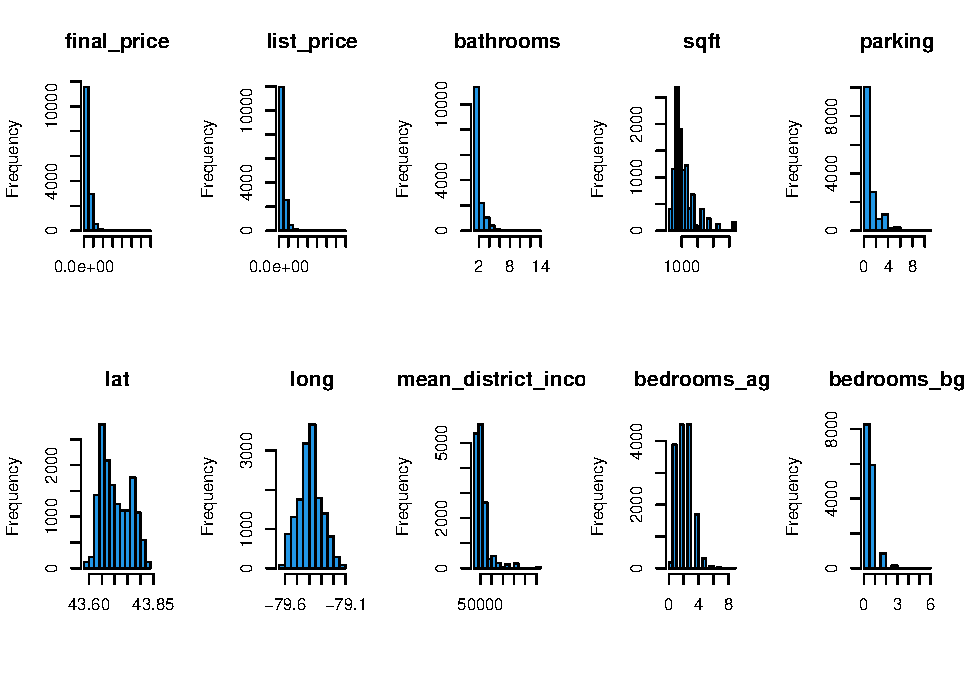
\includegraphics{R-markdown_sean_files/figure-latex/unnamed-chunk-2-1.pdf}

\hypertarget{discussion}{%
\section{Discussion}\label{discussion}}

\hypertarget{acknowledgements}{%
\section{Acknowledgements}\label{acknowledgements}}

The authors would like to thank Hashmat Rohian, adjunct faculty at York
University for supervision of the project. We also thank Slava Spirin
for the original extraction of the Toronto Housing dataset {[}1{]}.
Finally, we thank Steve V. Miller for creation of the manuscript
template in R Markdown {[}2{]}.

\hypertarget{references}{%
\section{References}\label{references}}

\noindent

\hypertarget{refs}{}
\leavevmode\hypertarget{ref-spirin_slavaspirintoronto-housing-price-prediction_2020}{}%
1. Spirin, S. (2020). Slavaspirin/toronto-housing-price-prediction
Available at:
\url{https://github.com/slavaspirin/Toronto-housing-price-prediction}
{[}Accessed October 26, 2020{]}.

\leavevmode\hypertarget{ref-miller_r_nodate}{}%
2. Miller, S.V. An r markdown template for academic manuscripts. Steven
v. Miller. Available at:
\url{http://svmiller.com/blog/2016/02/svm-r-markdown-manuscript/}
{[}Accessed October 26, 2020{]}.





\newpage
\singlespacing 
\end{document}
